\section{Aperçu}
    

Pour entamer cette exploration, il est essentiel de bien définir et comprendre la nature des threads. Dans son ouvrage intitulé « The Linux Programming Interface », on trouve une définition concise : « Like processes, threads are a mechanism that permits an application to perform multiple tasks concurrently. A single process can contain multiple threads. All of these threads independently execute the same program, and they all share the same global memory, including the initialized data, uninitialized data, and heap segments. ». Ce qui, en français, nous donne : « Comme les processus, les threads sont un mécanisme qui permet à une application d'effectuer plusieurs tâches simultanément. Un seul processus peut contenir plusieurs threads. Tous ces threads exécutent indépendamment le même programme et partagent la même mémoire globale, y compris les segments de données initialisées, non initialisées et du tas. ». Bien que cette définition apporte des éclaircissements, certaines zones demeurent encore floues et nécessitent une clarification approfondie. Nous allons donc examiner de plus près ces aspects ambigus pour consolider nos bases.



\section{Introduction au concept de Thread}
Tout d’abord, partons d’une base connue et acquise : les processus Linux. Comme nous le savons bien, un processus sous Linux nous permet d’effectuer différentes actions les unes à la suite des autres. Par exemple, afficher à l’écran un message d’accueil, puis demander à l’utilisateur une entrée, attendre la réponse de l’utilisateur et enfin traiter cette réponse. Comme nous pouvons le constater, il s’agit ici d’une approche séquentielle de l’exécution des instructions. On va d'abord afficher le message à l’écran, ensuite on va attendre l’entrée de l’utilisateur. Pendant cette attente, le processus n’effectue rien car il attend la fin de l’entrée de l’utilisateur. Enfin, dès que l’utilisateur a fini son entrée, le processus peut reprendre et traiter l’information. Voici une limitation de l’implémentation de base des processus sous Linux.

Si nous souhaitons toutefois faire plusieurs choses en même temps, des solutions sont à notre disposition.

La première solution consiste à utiliser la commande \textit{fork()} afin de créer un nouveau processus et lui donner une tâche spécifique. Bien que cette méthode présente de nombreux avantages, elle contient également son lot de désavantages, tels que le coût en performances de la commande \textit{fork()} qui copie la quasi-totalité du processus parent. De plus, le partage des données en mémoire devient plus complexe car dans le cas d’un clone, nous devrons utiliser un pipe pour communiquer entre parent et enfant, et dans le cas de différents processus, nous devons utiliser une zone de mémoire partagée.

\begin{figure}[ht]
  \centering
  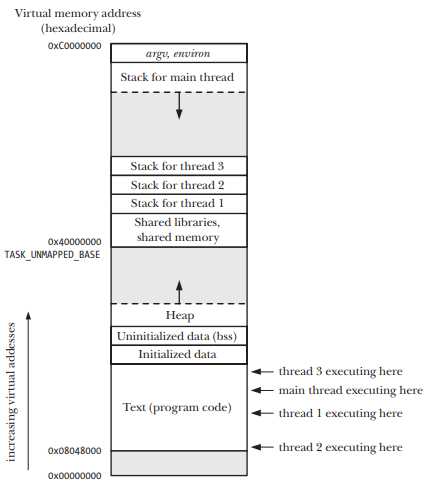
\includegraphics[width=0.8\linewidth]{thread_memory.png}
  \caption{Espace mémoire de threads}
  \label{fig:thread_memory}
\end{figure}
\vspace{\baselineskip}

Entre alors en jeu les threads. Leur création est bien moins gourmande, car tous les threads d’un même processus partagent de nombreux attributs entre eux, ce qui augmente fortement les performances car moins de données sont copiées. En effet, selon le livre \href{file:///C:/Users/rochk/Downloads/The%20Linux%20Programming%20Interface-Michael%20Kerrisk.pdf}{The Linux Programming Interface}, la création d'un thread serait 10 fois plus rapide, voire plus, que la création d'un processus. Malheureusement, cela apporte également son lot de problèmes à gérer, comme l’accès aux données par deux threads. Nous aborderons ce sujet plus en détail plus bas dans le document.
\\
\begin{figure}[ht]
    \centering
    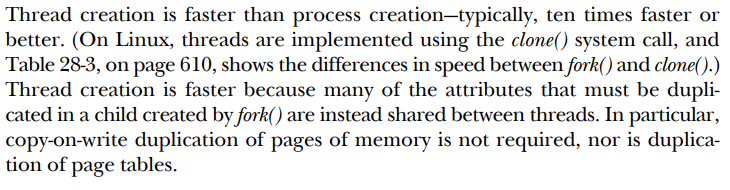
\includegraphics[width=0.9\linewidth]{thread_creation.png}
    \caption{Rapidité création thread}
    \label{fig:thread_creation}
\end{figure}
\vspace{\baselineskip}

Comme nous l’avons énoncé plus haut, un processus peut contenir plusieurs threads qui s’exécutent simultanément. Nous allons maintenant voir ce que contient un thread et comment il interagit avec le processus. Tout d’abord, un thread est composé de plusieurs attributs, entre autres : un ID de thread, un contexte d'exécution, une pile et un ensemble de registres.
Ce qui nous intéressera dans cette recherche sont l'ID du thread et sa pile. Les threads partagent entre eux : l’espace d’adressage mémoire, le code du programme, le tas, les variables d’environnement, les descripteurs de fichier ainsi que le gestionnaire de signaux. Par contre, ce qu’ils ne partagent pas sont : la pile d’exécution, le gestionnaire d’exception, la priorité d’ordonnancement, le stockage local ainsi que les identifiants.
\\

Maintenant que nous savons à quoi nous avons affaire, penchons-nous sur le fonctionnement des threads au sein du processus. Il ne nous faudra pas chercher bien loin, car nous les utilisions inconsciemment depuis le début. En effet, dès le démarrage, un processus s’exécute sur son thread principal, ce que l’on appelle un processus traditionnel ou « heavyweight process ». C’est sur ce thread principal que s’exécutent toutes les instructions écrites dans le code du processus. Lorsque nous ajoutons des threads supplémentaires à notre processus, nous basculons alors dans un processus multithread. Grâce à cela, nous pouvons maintenant effectuer plusieurs actions simultanément sans devoir attendre l’accomplissement de l’instruction précédente.
\\

